\section{Componenti e classi}
	\subsection{Romeo}
		\subsubsection{Informazioni sul package}
			\begin{figure}[!h]
				\centering
				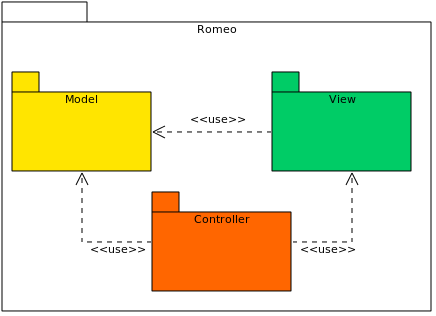
\includegraphics[scale=0.5]{./Content/Immagini/Romeo.png}
				\caption{Diagramma package \textsl{Romeo}}
			\end{figure}
			\paragraph{Descrizione:}Il package\g{} \textsl{Romeo} rappresenta il package\g{} globale del progetto. Le relazioni tra i package\g{} \textsl{Model}, \textsl{View} e \textsl{Controller}, rappresentano le relazioni tipiche del design pattern\g{} MVC\g{}.
			\paragraph{Package contenuti:}
				\begin{itemize}
					\item Romeo::Controller
					\item Romeo::Model
					\item Romeo::View
				\end{itemize}
			\paragraph{Relazioni d'uso tra i componenti}
COMPLETAREEEEEEEEE	\subsection{Romeo::Controller}
		\subsubsection{Informazioni sul package}
			\begin{figure}[!h]
				\centering
				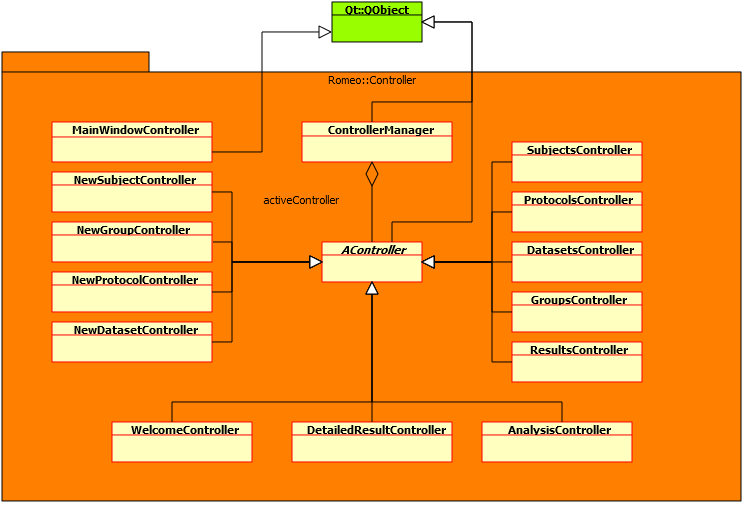
\includegraphics[scale=0.5]{./Content/Immagini/Romeo__Controller.png}
				\caption{Diagramma package \textsl{Romeo::Controller}}
			\end{figure}
			\paragraph{Descrizione:}Package\g{} rappresentante la componente \textsl{Controller} dell'architettura MVC\g{}.
			\paragraph{Relazioni d'uso tra i componenti}
COMPLETAREEEEEEEEE		\subsubsection{Classi astratte contenute}
			\paragraph{\underline{AController}}
				\subparagraph{Descrizione:}Classe astratta che rappresenta un generico controller per un oggetto derivato dalla classe \textsl{APanel}
				\subparagraph{Contesto di utilizzo:}Riceve i signal\g{} dalla vista che sta gestendo e reagisce di conseguenza.
				\subparagraph{Ereditata da:}
					\begin{itemize}
						\item Romeo::Controller::DatasetsController
						\item Romeo::Controller::GroupsController
						\item Romeo::Controller::WelcomeController
					\end{itemize}
		\subsubsection{Classi contenute}
			\paragraph{\underline{ControllerManager}}
				\subparagraph{Descrizione:}Classe che si occupa di cancellare i controller dalla memoria, quando non sono più necessari. È implementata tramite il design patterng\g{} Singleton.
				\subparagraph{Contesto di utilizzo:}Si occupa di gestire ed eliminare i controller.
				\subparagraph{Eredita da:}
					\begin{itemize}
						\item Qt::QObject
					\end{itemize}
			\paragraph{\underline{DatasetsController}}
				\subparagraph{Descrizione:}Classe che rappresenta un controller per un oggetto di tipo \textsl{DatasetsView}.
				\subparagraph{Contesto di utilizzo:}Gestisce i signal\g{} emessi da un oggetto \textsl{DatasetsView} ed agisce conseguentemente in modo appropriato.
				\subparagraph{Eredita da:}
					\begin{itemize}
						\item Romeo::Controller::AController
					\end{itemize}
			\paragraph{\underline{GroupsController}}
				\subparagraph{Descrizione:}Classe che rappresenta un controller per un oggetto di tipo \textsl{GroupsView}.
				\subparagraph{Contesto di utilizzo:}Gestisce i signal\g{} emessi da un oggetto \textsl{GroupsView} ed agisce conseguentemente in modo appropriato.
				\subparagraph{Eredita da:}
					\begin{itemize}
						\item Romeo::Controller::AController
					\end{itemize}
			\paragraph{\underline{WelcomeController}}
				\subparagraph{Descrizione:}Classe che rappresenta un controller per un oggetto di tipo \textsl{WelcomeView}.
				\subparagraph{Contesto di utilizzo:}Gestisce i signal\g{} emessi da un oggetto \textsl{WelcomeView} ed agisce conseguentemente in modo appropriato.
				\subparagraph{Eredita da:}
					\begin{itemize}
						\item Romeo::Controller::AController
					\end{itemize}
	\subsection{Romeo::Model}
		\subsubsection{Informazioni sul package}
			\begin{figure}[!h]
				\centering
				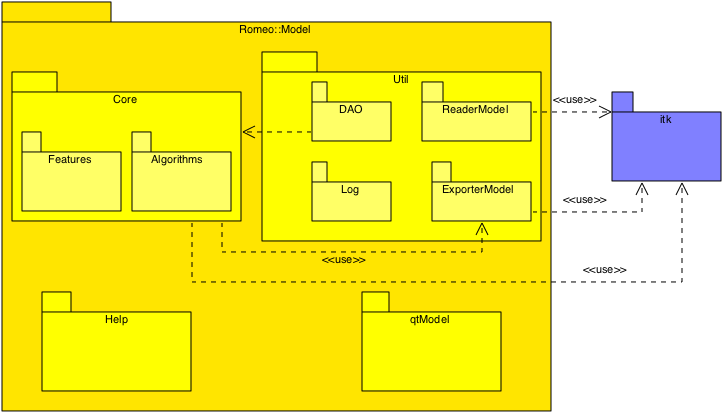
\includegraphics[scale=0.5]{./Content/Immagini/Romeo__Model.png}
				\caption{Diagramma package \textsl{Romeo::Model}}
			\end{figure}
			\paragraph{Descrizione:}Package\g{} rappresentante il componente \textsl{Model} dell'architettura MVC\g{}.
			\paragraph{Package contenuti:}
				\begin{itemize}
					\item Romeo::Model::Core
					\item Romeo::Model::Help
					\item Romeo::Model::qtModel
					\item Romeo::Model::Util
				\end{itemize}
			\paragraph{Relazioni d'uso tra i componenti}
COMPLETAREEEEEEEEE	\subsection{Romeo::Model::Core}
		\subsubsection{Informazioni sul package}
			\begin{figure}[!h]
				\centering
				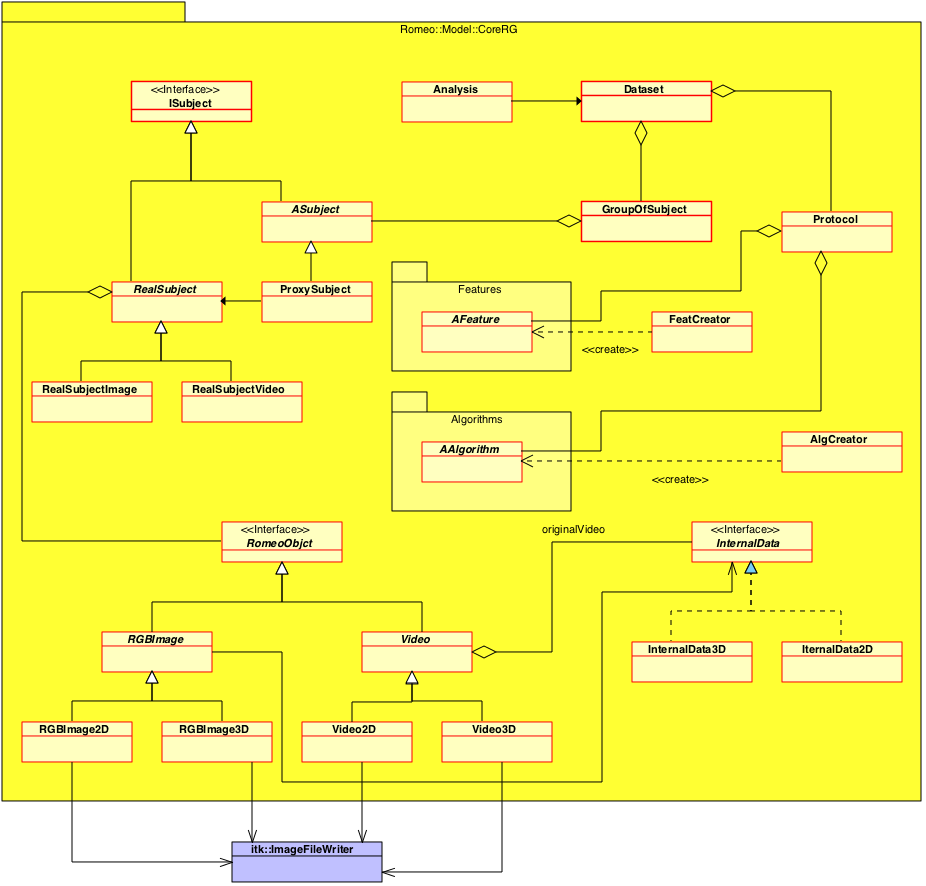
\includegraphics[scale=0.5]{./Content/Immagini/Romeo__Model__Core.png}
				\caption{Diagramma package \textsl{Romeo::Model::Core}}
			\end{figure}
			\paragraph{Descrizione:}Package\g{} contenente le classi rappresentanti le funzionalità principali del software. In questo package\g{} verrà utilizzato il design pattern\g{} Adapter, il quale consente di utilizzare alcune funzionalità offerte dalle librerie esterne.
			\paragraph{Package contenuti:}
				\begin{itemize}
					\item Romeo::Model::Core::Algorithms
					\item Romeo::Model::Core::Features
				\end{itemize}
			\paragraph{Relazioni d'uso tra i componenti}
COMPLETAREEEEEEEEE	\subsection{Romeo::Model::Core::Algorithms}
		\subsubsection{Informazioni sul package}
			\begin{figure}[!h]
				\centering
				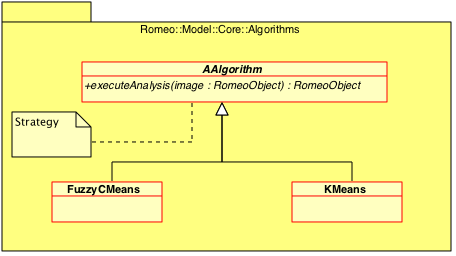
\includegraphics[scale=0.5]{./Content/Immagini/Romeo__Model__Core__Adapters__Algorithms.png}
				\caption{Diagramma package \textsl{Romeo::Model::Core::Algorithms}}
			\end{figure}
			\paragraph{Descrizione:}Package\g{} contenente le classi che permettono al \textsl{Model} di utilizzare gli algoritmi di clustering\g{} previsti nei requisiti. Le classi di questo package\g{} sono implementate utilizzando il design pattern\g{} Strategy.
			\paragraph{Relazioni d'uso tra i componenti}
COMPLETAREEEEEEEEE	\subsection{Romeo::Model::Core::Features}
		\subsubsection{Informazioni sul package}
			\begin{figure}[!h]
				\centering
				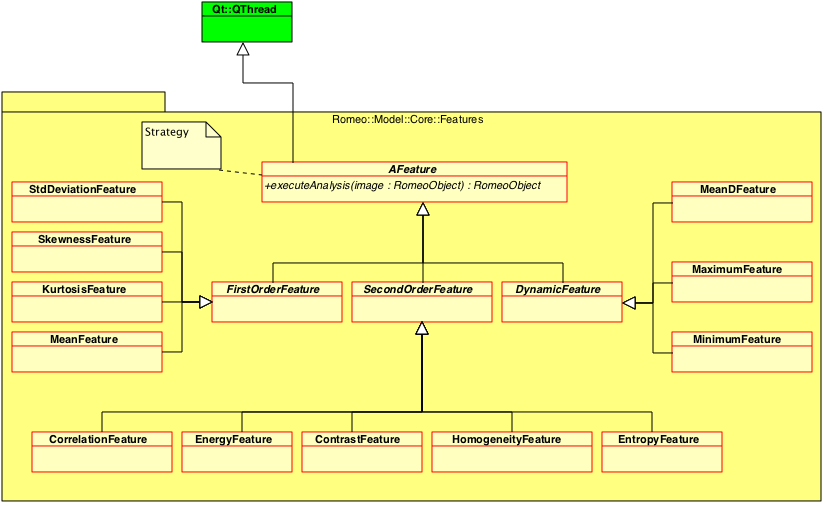
\includegraphics[scale=0.5]{./Content/Immagini/Romeo__Model__Core__Adapters__Features.png}
				\caption{Diagramma package \textsl{Romeo::Model::Core::Features}}
			\end{figure}
			\paragraph{Descrizione:}Package\g{} contenente le classi che permettono al \textsl{Model} di utilizzare le features\g{} previste nei requisiti. Le classi di questo package\g{} sono implementate usando il design pattern\g{} Strategy.
			\paragraph{Relazioni d'uso tra i componenti}
COMPLETAREEEEEEEEE	\subsection{Romeo::Model::Help}
		\subsubsection{Informazioni sul package}
			\begin{figure}[!h]
				\centering
				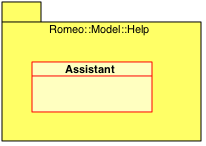
\includegraphics[scale=0.5]{./Content/Immagini/Help.png}
				\caption{Diagramma package \textsl{Romeo::Model::Help}}
			\end{figure}
			\paragraph{Descrizione:}Package\g{} contenente la classe dedicata a caricare il contenuto dei file riguardanti la guida utente.
			\paragraph{Relazioni d'uso tra i componenti}
COMPLETAREEEEEEEEE	\subsection{Romeo::Model::qtModel}
		\subsubsection{Informazioni sul package}
			\begin{figure}[!h]
				\centering
				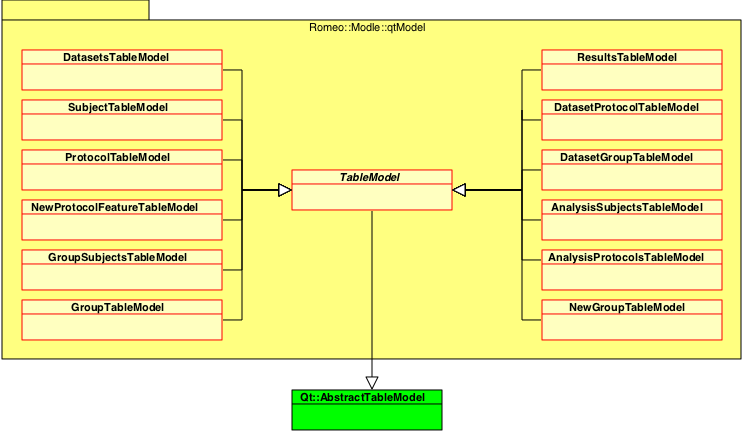
\includegraphics[scale=0.5]{./Content/Immagini/Romeo__Model__qtModel.png}
				\caption{Diagramma package \textsl{Romeo::Model::qtModel}}
			\end{figure}
			\paragraph{Descrizione:}Package\g{} contenente le classi che estendono i \textsl{Model} per le tabelle e liste proprietari di Qt\g{}, utilizzate delle \textsl{QTableView} e \textsl{QListView} presenti nelle viste.
			\paragraph{Relazioni d'uso tra i componenti}
COMPLETAREEEEEEEEE	\subsection{Romeo::Model::Util}
		\subsubsection{Informazioni sul package}
			\begin{figure}[!h]
				\centering
				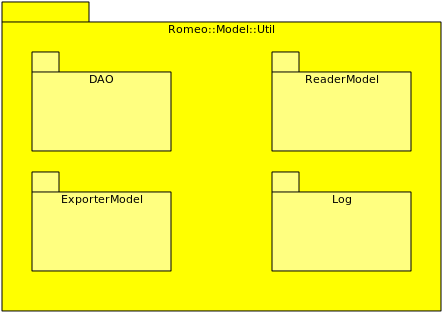
\includegraphics[scale=0.5]{./Content/Immagini/Romeo__Model__Util.png}
				\caption{Diagramma package \textsl{Romeo::Model::Util}}
			\end{figure}
			\paragraph{Descrizione:}L'obiettivo di questo package\g{} è quello di fornire una serie di classi di utilità e di supporto per le funzionalità core dell'applicativo.
			\paragraph{Package contenuti:}
				\begin{itemize}
					\item Romeo::Model::Util::DAO
					\item Romeo::Model::Util::ExporterModel
					\item Romeo::Model::Util::Log
					\item Romeo::Model::Util::ReaderModel
				\end{itemize}
			\paragraph{Relazioni d'uso tra i componenti}
COMPLETAREEEEEEEEE	\subsection{Romeo::Model::Util::DAO}
		\subsubsection{Informazioni sul package}
			\begin{figure}[!h]
				\centering
				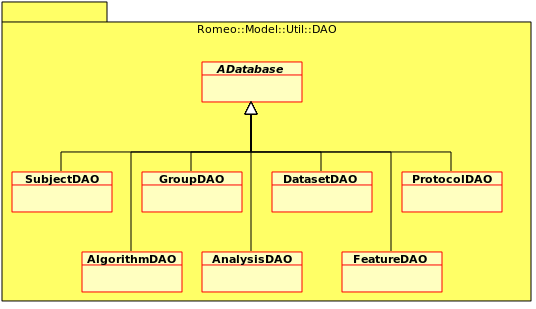
\includegraphics[scale=0.5]{./Content/Immagini/DAO.png}
				\caption{Diagramma package \textsl{Romeo::Model::Util::DAO}}
			\end{figure}
			\paragraph{Descrizione:}Package\g{} che gestisce l'interfacciamento con il database del sistema\footnote{Per maggiori informazioni vedere la sezione \ref{DB}}. Per ogni tabella del database è stata creata un una classe che estende la classe astratta \hyperref[dao::adatabase]{\textsl{ADatabase}}.
			\paragraph{Relazioni d'uso tra i componenti}
COMPLETAREEEEEEEEE	\subsection{Romeo::Model::Util::ExporterModel}
		\subsubsection{Informazioni sul package}
			\begin{figure}[!h]
				\centering
				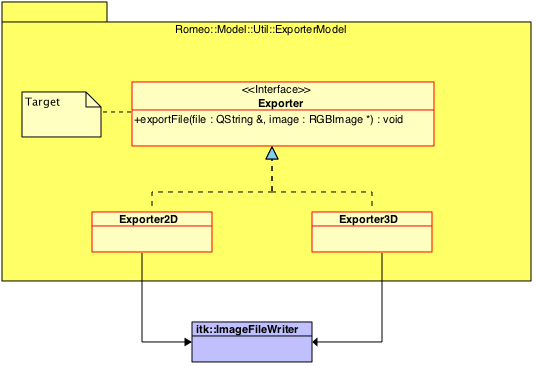
\includegraphics[scale=0.5]{./Content/Immagini/ExporterModel.png}
				\caption{Diagramma package \textsl{Romeo::Model::Util::ExporterMod}}
			\end{figure}
			\paragraph{Descrizione:}Package\g{} contenente le classi che si occupano di trasformare le immagini dal formato interno usato per l'analisi, al formato desiderato dall'utente, tra quelli previsti dai requisiti. Le classi di questo package\g{} sono implementate tramite il design pattern\g{} Adapter utilizzando le classi fornite dalla libreria esterna ITK\g{}.
			\paragraph{Relazioni d'uso tra i componenti}
COMPLETAREEEEEEEEE	\subsection{Romeo::Model::Util::Log}
		\subsubsection{Informazioni sul package}
			\begin{figure}[!h]
				\centering
				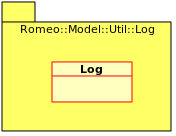
\includegraphics[scale=0.5]{./Content/Immagini/Romeo__Model__Util__Log.png}
				\caption{Diagramma package \textsl{Romeo::Model::Util::Log}}
			\end{figure}
			\paragraph{Descrizione:}Package\g{} contenente la classe che si occupa di gestire e produrre dei file di log, nei quali saranno contenute informazioni utili agli sviluppatori.
			\paragraph{Relazioni d'uso tra i componenti}
COMPLETAREEEEEEEEE	\subsection{Romeo::Model::Util::ReaderModel}
		\subsubsection{Informazioni sul package}
			\begin{figure}[!h]
				\centering
				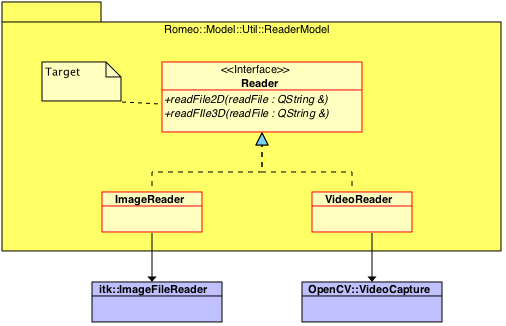
\includegraphics[scale=0.5]{./Content/Immagini/Romeo__Model__Util__ReaderModel.png}
				\caption{Diagramma package \textsl{Romeo::Model::Util::ReaderModel}}
			\end{figure}
			\paragraph{Descrizione:}Package\g{} contenente le classi che si occupano di leggere le immagini e trasformarle nel formato interno usato all'interno di \project{}. Le classi di questo package\g{} sono implementate tramite il design pattern\g{} Adapter adattando le classi fornite dalla libreria esterna ITK\g{}.
			\paragraph{Relazioni d'uso tra i componenti}
COMPLETAREEEEEEEEE	\subsection{Romeo::View}
		\subsubsection{Informazioni sul package}
			\begin{figure}[!h]
				\centering
				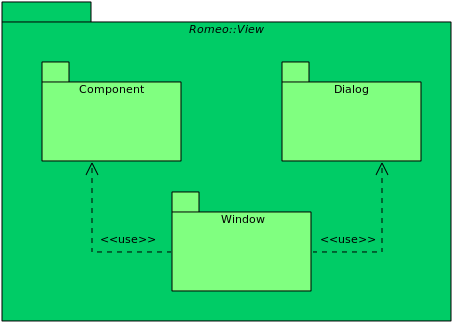
\includegraphics[scale=0.5]{./Content/Immagini/Romeo__View.png}
				\caption{Diagramma package \textsl{Romeo::View}}
			\end{figure}
			\paragraph{Descrizione:}Package\g{} che rappresenta la componente \textsl{View} dell'architettura MVC\g{}.
			\paragraph{Package contenuti:}
				\begin{itemize}
					\item Romeo::View::Component
					\item Romeo::View::Dialog
					\item Romeo::View::Window
				\end{itemize}
			\paragraph{Relazioni d'uso tra i componenti}
COMPLETAREEEEEEEEE	\subsection{Romeo::View::Component}
		\subsubsection{Informazioni sul package}
			\begin{figure}[!h]
				\centering
				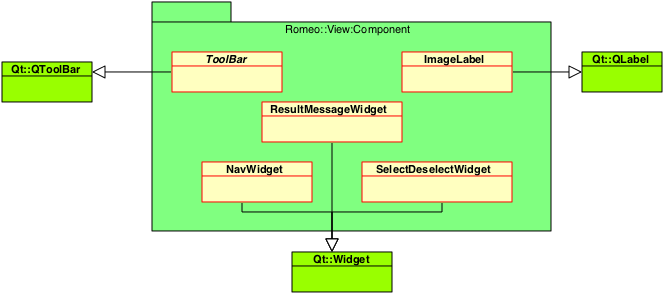
\includegraphics[scale=0.5]{./Content/Immagini/Romeo__View__Component.png}
				\caption{Diagramma package \textsl{Romeo::View::Component}}
			\end{figure}
			\paragraph{Descrizione:}Package\g{} contenente le classi comuni a tutte le viste.
			\paragraph{Relazioni d'uso tra i componenti}
COMPLETAREEEEEEEEE	\subsection{Romeo::View::Dialog}
		\subsubsection{Informazioni sul package}
			\begin{figure}[!h]
				\centering
				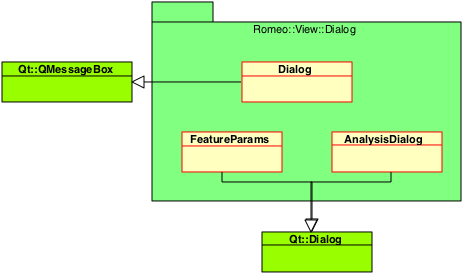
\includegraphics[scale=0.5]{./Content/Immagini/Romeo__View__Dialog.png}
				\caption{Diagramma package \textsl{Romeo::View::Dialog}}
			\end{figure}
			\paragraph{Descrizione:}Package\g{} contenente l'insieme delle classi che gestiscono le finestre di dialogo con le quali l'utente può interagire con \project{}.
			\paragraph{Relazioni d'uso tra i componenti}
COMPLETAREEEEEEEEE	\subsection{Romeo::View::Window}
		\subsubsection{Informazioni sul package}
			\begin{figure}[!h]
				\centering
				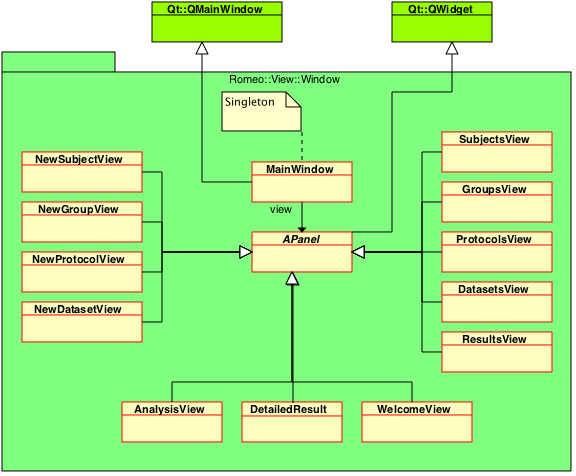
\includegraphics[scale=0.5]{./Content/Immagini/Window.png}
				\caption{Diagramma package \textsl{Romeo::View::Window}}
			\end{figure}
			\paragraph{Descrizione:}Package\g{} contenente l'insieme delle finestre con le quali l'utente può interagire durante l'esecuzione di \project{}.
			\paragraph{Relazioni d'uso tra i componenti}
COMPLETAREEEEEEEEE